\ifx\allfiles\undefined
\documentclass[12pt, a4paper, oneside, UTF8]{ctexbook}
\def\path{../../config}
\usepackage{amsthm}
\usepackage{amssymb}
\usepackage{array}
\usepackage{xcolor}
\usepackage{graphicx}
\usepackage{mathrsfs}
\usepackage{enumitem}
\usepackage{geometry}
\usepackage[colorlinks, linkcolor=black]{hyperref}
\usepackage{stackengine}
\usepackage{yhmath}
\usepackage{extarrows}
\usepackage{tikz}
\usepackage{forest}
\usetikzlibrary{decorations.pathreplacing, positioning}
% \usepackage{unicode-math}
\usepackage{esint}
\usepackage{pifont}
\usepackage{tcolorbox}
\tcbuselibrary{skins, breakable}

\usepackage{multicol} 
\usepackage{fontspec} % 使用字体

\setmainfont{Times New Roman}
\setCJKmainfont{LXGWWenKai-Light}[
    SlantedFont=*
]

\usepackage{listings} % 用于插入代码

% 定义代码高亮风格
\lstset{
    basicstyle=\ttfamily\small,        % 基本字体样式(等宽小字体)
    keywordstyle=\color{blue},         % 关键字颜色
    commentstyle=\color{green},        % 注释颜色
    stringstyle=\color{red},           % 字符串颜色
    numbers=none,
    breaklines=true,                   % 自动换行
    frame=single,                      % 代码框边框
    rulecolor=\color{black},           % 边框颜色
    captionpos=b,                      % 标题位置(底部)
    showspaces=false,                  % 不显示空格标记
    showstringspaces=false,            % 不显示字符串中的空格标记
    language=C                         % 设置语言为 C
}

\usepackage{fontawesome5}

\usepackage{amsmath}
\usepackage{booktabs, array}
\usepackage{makecell}
\usepackage{fancyhdr}
\usepackage[dvipsnames, svgnames]{xcolor}
\usepackage{listings}
\usepackage{tasks}[2020/01/11]

\everymath{\displaystyle}

\definecolor{mygreen}{rgb}{0,0.6,0}
\definecolor{mygray}{rgb}{0.5,0.5,0.5}
\definecolor{mymauve}{rgb}{0.58,0,0.82}
\definecolor{NavyBlue}{RGB}{0,0,128}
\definecolor{Rhodamine}{RGB}{255,0,255}
\definecolor{PineGreen}{RGB}{0,128,0}

\graphicspath{ {figures/},{../figures/}, {config/}, {../config/} }

\linespread{1.6}

\geometry{
    top=25.4mm, 
    bottom=25.4mm, 
    left=20mm, 
    right=20mm, 
    headheight=2.17cm, 
    headsep=4mm, 
    footskip=12mm
}

\setenumerate[1]{itemsep=5pt,partopsep=0pt,parsep=\parskip,topsep=5pt}
\setitemize[1]{itemsep=5pt,partopsep=0pt,parsep=\parskip,topsep=5pt}
\setdescription{itemsep=5pt,partopsep=0pt,parsep=\parskip,topsep=5pt}



% \begin{lstlisting}[language=TeX] ... \end{lstlisting}

% 定理环境设置
% ---------- 颜色 ----------
\definecolor{ExBlue}{HTML}{4F81BD}
\definecolor{SolGreen}{HTML}{77933C}
\definecolor{DefRed}{HTML}{C5504B}
\definecolor{ThmOrange}{HTML}{E97132}
\definecolor{RemGray}{HTML}{7F7F7F}
\definecolor{CorPurple}{HTML}{7030A0}
\definecolor{ForGray}{HTML}{595959}

% ---------- 通用“变色”模板 ----------
\tcbset{
    mybox/.style n args={1}{
        enhanced, breakable,
        arc=6pt,
        boxrule=0.6pt,
        left=8pt, right=8pt, top=6pt, bottom=6pt,
        drop shadow={black!25},
        fonttitle=\bfseries,
        coltitle=white,
        colbacktitle=#1!85,
        colback=#1!10,
        colframe=#1,
    }
}

% ---------- 各环境 ----------
% 例题
\newtcolorbox{example}[1][]{mybox={ExBlue}, title={\ifstrempty{#1}{Example}{#1}}}
% 解答
\newtcolorbox{solution}[1][]{mybox={SolGreen}, title={\ifstrempty{#1}{Solution}{#1}}}
% 定义
\newtcolorbox{definition}[1][]{mybox={DefRed}, title={\ifstrempty{#1}{Definition}{#1}}}
% 定理
\newtcolorbox{theorem}[1][]{mybox={ThmOrange}, title={\ifstrempty{#1}{Theorem}{#1}}}
% 标注
\newtcolorbox{remark}[1][]{mybox={RemGray}, title={\ifstrempty{#1}{Remark}{#1}}}
% 推论
\newtcolorbox{corollary}[1][]{mybox={CorPurple}, title={\ifstrempty{#1}{Corollary}{#1}}}
% 公式
\newtcolorbox{formula}[1][]{mybox={ForGray}, title={\ifstrempty{#1}{Formula}{#1}}}


\settasks{
    label-format = \bfseries,
    label        = \Alph*.,
    label-width  = 1.2em,
    label-offset = 0.3em,
    item-indent  = 1.9em,
    column-sep   = 0.5em
}

\newenvironment{choices}[1][4]   % 默认 4 栏
    {\begin{tasks}(#1)}
    {\end{tasks}}

% 自定义命令的文件

\def\d{\mathrm{d}}
\def\R{\mathbb{R}}
\def\P{\partial} 
\newcommand{\bs}[1]{\begin{solution}#1\end{solution}}
\newcommand{\bt}[1][1]{% 默认参数为1
    \ensuremath{% 确保数学模式
        \foreach \n in {1,...,#1} {\blacktriangle}% 循环输出 #1 个黑色三角形
    }%
}

\newcommand{\bl}[1][1]{% 默认参数为1
    \ensuremath{% 确保数学模式
        \foreach \n in {1,...,#1} {\blacklozenge}% 循环输出 #1 个黑色三角形
    }%
}
\newif\ifshowanswers
%\showanswerstrue % 注释掉这行就不显示答案

% 定义答案环境
\newcommand{\answer}[1]{%
    \ifshowanswers
        #1%
    \fi
}




% 修改参数改变封面样式,0 默认原始封面、内置其他1、2、3种封面样式
\def\myIndex{3}


\ifnum\myIndex>0
    \input{\path/cover_package_\myIndex} 
\fi

\def\myTitle{冲刺150笔记}
\def\myAuthor{Weary Bird}
\def\myDateCover{\today}
\def\myDateForeword{\today}
\def\myForeword{行香子}
\def\myForewordText{
树绕村庄,水满陂塘;倚东风、豪兴徜徉。小园几许,收尽春光。有桃花红,李花白,菜花黄。 \\
远远苔墙,隐隐茅堂;飏青旗、流水桥旁。偶然乘兴,步过东冈。正莺儿啼,燕儿舞,蝶儿忙。 \\
}
\def\mySubheading{知错能改善莫大焉}


\begin{document}
% \input{../config/cover}
\else
\fi

\chapter{一维随机变量}

\section{分布函数的判定与计算}
\begin{remark}
    (分布函数的性质)
    \item [(1)] $0\leq F(x)\leq 1, -\infty < x < +\infty, F(-\infty) = 0, F(+\infty)=1$ 
    \item [(2)] (单调不减) 当$x_1 < x_2$时,$F(x_1)<F(x_2)$ 
    \item [(3)] (右连续) $F(x+0)=F(x)$ \\
    上面三个性质为分布函数的定义,只要满足上述性质的函数一定是某一个概率分布的分布函数
    \item [(4)] $P\{a<X\leq b\}=F(b)-F(a)$
    \item [(5)] $P\{X<x\}=F(x-0), P\{X=x\}=F(x)-F(x-0)$ \\
    $P\{a\leq x\leq b\}=P\{x\leq b\}-P\{x<a\}=F(b)-F(a-0)$ \\
    $P\{a<x<b\}=P\{x<b\}-P\{x\leq a\}=F(b-0)-F(a)$
\end{remark}

\begin{enumerate}[label=\arabic*.]
    % 例题2.1
    \item 设随机变量$X$的分布函数为$F(x)$,$a,b$为任意常数,则下列一定不是分布函数的是
    \begin{align*}
        (A)\ F(ax+b) \quad (B)\ F(ax^2+b) \quad (C)\ F(ax^3+b) \quad (D)\ 1-F(-x)
    \end{align*}
    
    \begin{tcolorbox}[title=总结]
        对于$F(ax+b),F(ax^3+b),\ldots$只要$a>0$则这些函数都是分布函数 \\
        对于$F(a^2x+b),F(a^4+b),\ldots$都一定不是分布函数 \\
        对于$G(x)=1-F(-x)$ 
        \\若$X$是连续性随机变量则是,否则不是($F(x)$不满足左连续,则$G(x)$不满足右连续)
    \end{tcolorbox}
    
    \item 设随机变量$X$的概率密度为
    % 例题2.2
    \[
        f(x)=
        \begin{cases}
            1-|x|, & |x|<1 \\
            0, & \text{其他}
        \end{cases}
    \]
    则$X$的分布函数$F(x)=$\_\_\_\_,$P\{-2<X<\frac{1}{4}\}=$\_\_\_\_.
    
    \begin{solution}
    \item [(方法一 变限积分)]
        \[
        f(x)=
        \begin{cases}
            1 + x ,&  -1 < x < 0 \\
            1 - x, & 0 \leq x < 1 \\
            0, &\text{其他情况}
        \end{cases}
        \]
        根据 $F(x) = \int_{-\infty}^{x}f(t)\, \mathrm{d}t$,有
        \begin{align*}
        F(x) &=
        \begin{cases}
            0, & x \leq -1 \\
            \int_{-1}^{x}(1 + t)\, \mathrm{d}t, &  -1 < x < 0 \\
            \int_{-1}^{0}(1 + t)\, \mathrm{d}t + \int_{0}^{x}(1 - t)\, \mathrm{d}t, & 0 \leq x < 1 \\
            1, & x \geq 1 
        \end{cases} \\
        &= \begin{cases}
            0, & x \leq -1 \\
            x+\frac{x^2}{2}+\frac{1}{2}, &  -1 < x < 0 \\
            x-\frac{x^2}{2}+\frac{1}{2}, & 0 \leq x < 1 \\
            1, & x \geq 1 
        \end{cases} \\
        P\{-2< X < \frac{1}{4}\} &= F(\frac{1}{4}) - F(-2) \\
        &= \int_{-2}^{\frac{1}{4}} f(x)\d x \\
        &=\frac{23}{32}
        \end{align*}
    \item [(方法二 定积分)]
    \begin{align*}
    \int f(x)\d x &= \begin{cases}
        C_1, & x < -1 \\
        x+\frac{x^2}{2}+C_2, & -1 \leq x < 0 \\
        x-\frac{x^2}{2}+C_3, & 0 \leq x < 1 \\
        C_4, & x \geq 1 
    \end{cases} \\
    &\xlongequal{\text{由分布函数的定义}}{}\begin{cases}
        0, & x \leq -1 \\
        x+\frac{x^2}{2}+\frac{1}{2}, &  -1 < x < 0 \\
        x-\frac{x^2}{2}+\frac{1}{2}, & 0 \leq x < 1 \\
        1, & x \geq 1 
        \end{cases}
    \end{align*}
    \end{solution}
\end{enumerate}

\section{概率密度的判定与计算}
\begin{remark}
    (概率密度的性质)
    \item [(1)] $f(x)\geq 0, -\infty < x +\infty$ 
    \item [(2)] $\int_{-\infty}^{+\infty}f(x)\d x = 1$ \\
    上面两条性质为概率密度的定义,任何满足上面的函数都是某个概率的概率密度函数 
    \item [(3)] $P\{a<X\leq b\}=\int_{a}^{b}f(x)\d x$ \\
    推广$P\{a<X\leq b\}=P\{a\leq X\leq b\}=P\{a\leq X < b\} = P\{a<X <  b\} =\int_{a}^{b}f(x)\d x$ 
    \item [(4)] 在$f(x)$\textbf{连续点}处有$F'(x)=f(x)$ 
\end{remark}
\begin{enumerate}[label=\arabic*.,start=3]
    % 例题2.3
    \item 设随机变量$X$的概率密度为$f(x)$,则下列必为概率密度的是
    \begin{align*}
        (A)\ f(-x+1) \quad (B)\ f(2x-1) \quad (C)\ f(-2x+1) \quad (D)\ f\left(\frac{1}{2}x-1\right)
    \end{align*}
    
    \begin{solution}
    由于$f(x)$已经满足非负性,故选项的非负性都不需要考虑,只需要考虑正则性就可以. 
    \item [(A)] $\int_{-\infty}^{+\infty}f(-x+1)dx = \int_{-\infty}^{+\infty}f(u)du = 1 $
    \item [(B)] $\int_{-\infty}^{+\infty}f(2x-1)dx = \frac{1}{2}\int_{-\infty}^{+\infty}f(u)du = \frac{1}{2} $
    \item [(C)] $\int_{-\infty}^{+\infty}f(-2x+1)dx =\frac{1}{2}\int_{-\infty}^{+\infty}f(u)du = \frac{1}{2} $
    \item [(D)] $\int_{-\infty}^{+\infty}f(\frac{1}{2} - 1)dx  = 2\int_{-\infty}^{+\infty}f(u)du = 2$
    \end{solution}
    
    \begin{tcolorbox}[title=总结]
        $f(ax+b)$为概率密度$\iff\left|a\right|=1$
    \end{tcolorbox}
    % 例题2.4
    \item (2011,数一、三)设$F_1(x),F_2(x)$为分布函数,对应的概率密度$f_1(x),f_2(x)$为连续函数,则下列必为概率密度的是
    \begin{align*}
        (A)\ f_1(x)f_2(x) \quad (B)\ 2f_2(x)F_1(x) \quad (C)\ f_1(x)F_2(x) \quad (D)\ f_1(x)F_2(x)+f_2(x)F_1(x)
    \end{align*}
    
    \begin{tcolorbox}[title=总结]
        (1)线性组合 \\
        $af_1(x)+bf_2(x),a>0,b>0$为概率密度$\iff a+b=1$ \\
        $aF_1(x)+bF_2(x),a>0,b>0$为分布函数$\iff a+b=1$ \\
        (2)乘积 \\
        $F_1F_2$一定是分布函数 \\
        $f_1f_2$不一定是概率论密度 \\
        (3)混搭 \\
        $f_1F_2+f_2F_1,2f_1F_1,2f_2F_2$是概率密度,其余都不是.
    \end{tcolorbox}

    \newpage
    % 例题2.5
    \item (2000,三)设随机变量$X$的概率密度为
    \begin{align*}
        f(x)=\begin{cases}
            \frac{1}{3}, & x\in[0,1] \\
            \frac{2}{9}, & x\in[3,6] \\
            0, & \text{其他}
        \end{cases}
    \end{align*}
    若$P\{X\geq k\}=\frac{2}{3}$,则$k$的取值范围是\_\_\_\_.
\begin{solution}
    如图所示,当且仅当$1\leq k\leq 3$时候$P(X\geq k)=\frac{2}{3}$ 
\end{solution}
\begin{center}
    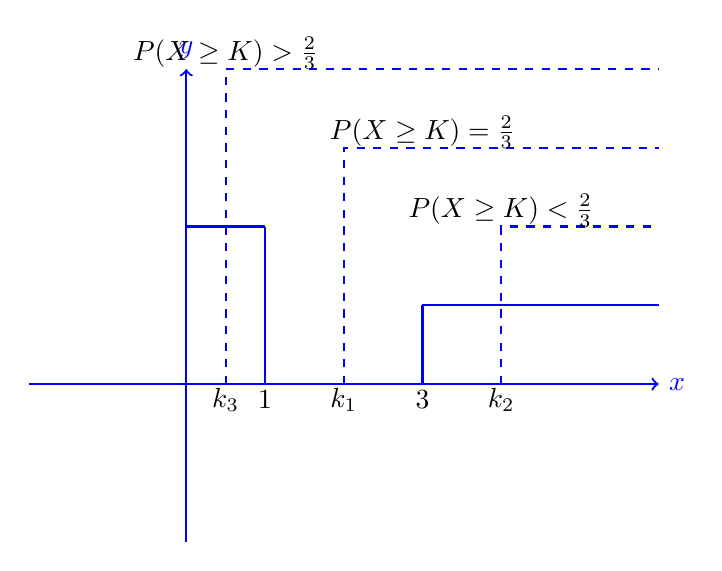
\begin{tikzpicture}
    % 绘制函数曲线
    \draw[blue, thick, ->] (-2,0) -- (6,0) node[right] {$x$};
    \draw[blue, thick, ->] (0,-2) -- (0,4) node[above] {$y$};
    \draw[blue, thick](0,2) -- (1,2);
    \draw[blue, thick](1,2) -- (1,0);
    \draw[blue, thick](3,1) -- (6,1);
    \draw[blue, thick](3,1) -- (3,0);

    \node at (1,-0.2) {$1$};
    \node at (3,-0.2) {$3$};


    \draw[blue, thick, dashed] (2,0)--(2,3)--(6,3);
    \node at (2,-0.2) {$k_1$};
    \node at (3,3.2) {$P(X\geq K)=\frac{2}{3}$};
    \draw[blue, thick, dashed] (4,0)--(4,2)--(6,2);
    \node at (4,-0.2) {$k_2$};
    \node at (4,2.2) {$P(X \geq K) < \frac{2}{3}$};
    \draw[blue, thick, dashed] (0.5,0)--(0.5,4)--(6,4);
    \node at (0.5,-0.2) {$k_3$};
    \node at (0.5,4.2) {$P(X \geq K)>\frac{2}{3}$};
    \end{tikzpicture}
\end{center}
\end{enumerate}

\section{关于八大分布}
\begin{remark}
    (八大分布的概率分布与数字特征)
    \item [(1)] 0-1分布, $X\sim B(1,p)$ 
    $
    \begin{array}{c|c c}
        X & 0 & 1\\
        \hline
        P & 1-p & p 
    \end{array}
    $, $EX=p, DX=p(1-p)$ 
    \item [(2)] 二项分布,$X\sim B(n,p)$ \newline
    $P\{X=k\}=C_n^{k}p^k(1-p)^{n-k},k=0,1,\ldots,n$,$EX=np, DX=np(1-p)$ 
    \item [(3)] 泊松分布,$X\sim P(\lambda)$ \\
    $P\{X=k\}=\frac{\lambda^k}{k!}e^{-\lambda},k=0,1,\ldots$, $EX=\lambda, DX=\lambda$ 
    \item [(4)] 几何分布,$X\sim G(p)$ \\
    $P=\{X=k\}=p(1-p)^{k-1},k=1,2,\ldots$, $EX=\frac{1}{p},DX=\frac{1-p}{p^2}$
    \item [(5)] 超几何分布,$X\sim H(N,M,n)$ \\
    $P=\{X=k\}=\frac{C_M^kC_{N-M}^{n-k}}{C_N^n},k=0,1,\ldots,min(n, M)$, $EX=\frac{nM}{N}$
    \item [(6)] 均匀分布 $X\sim U(a, b)$ \\
    $f(x)=\begin{cases}
        \frac{1}{b-a}, & a\leq x \leq b \\
        0, & \text{其他}
    \end{cases}$, 
    $F(x)=\begin{cases}
        0, & x < a \\
        \frac{x-a}{b-a}, &a\leq x < b \\
        1, & x \geq b
    \end{cases}
    $, $EX=\frac{a+b}{2},DX=\frac{(b-a)^2}{12}$ 
    \item [(7)] 指数分布 $X\sim E(\lambda)$ \\
    $f(x)=\begin{cases}
        \lambda e^{-\lambda x}, & x > 0 \\
        0, & x\leq 0 
    \end{cases}$, $\lambda > 0$
    $F(x)=\begin{cases}
        1-e^{-\lambda x}, & x > 0 \\
        0, & x\leq 0
    \end{cases}
    $, $EX=\frac{1}{\lambda}, DX=\frac{1}{\lambda ^ 2}$
    \item [(8)]  一般正态分布 $X \sim N(\mu,\sigma^{2})$,
    $EX=\mu, DX=\sigma^2$ \\
    $f(x)=\frac{1}{\sqrt{2\pi}\sigma}e^{-\frac{(x - \mu)^{2}}{2\sigma^{2}}}$,
    $F(\mu)=\frac{1}{2}$,
    $F(x)=\varPhi\left(\frac{x-\mu}{\sigma}\right)$ \\
    标准正态分布 $X \sim N(0,1)$ 
    $\varphi(x)=\frac{1}{\sqrt{2\pi}}e^{-\frac{x^{2}}{2}}$,
    $\varPhi(0)=\frac{1}{2}$,$\varPhi(-x)=1 - \varPhi(x)$ \\
    正态分布的标准化若$X \sim N(\mu,\sigma^{2})$,则 $\frac{X-\mu}{\sigma}\sim N(0,1)$.
\end{remark}

\myspace{1}
\begin{tcolorbox}[title=拓展-负二项分布]
    在一系列独立重复的伯努利试验(每次试验只有“成功”或“失败”两种结果,成功概率为 $p$)中,达到 $r$ 次成功所需的试验总次数 $X$ 服从负二项分布。\\
    $P(X=k)=\binom{k-1}{r-1}p^r(1-p)^{k-r},\quad k=r,r+1,r+2,\ldots,\quad EX=\frac{r}{p},\quad DX=\frac{r(1-p)}{p^2}$
\end{tcolorbox}
\begin{enumerate}[label=\arabic*.,start=6]
    % 例题2.6
    \item 设随机变量$X$的概率分布为$P\{X=k\}=C\frac{\lambda^k}{k!}$,$k=1,2,\cdots$,则$C=$\_\_\_\_.
    
    \begin{solution}
    \item[(方法一:级数)] 由概率的规范性可知$\sum_{k=1}^{\infty}C\frac{\lambda^k}{k!}=1$,由于
    $e^x=\sum_{i=0}^{\infty}\frac{x^n}{n!}$,故$C(e^{\lambda}-1)=1$,故$C=\frac{1}{e^{\lambda}-1}$
    \item [(方法二:泊松分布)] 考虑泊松分布$P\{X=k\}=\frac{\lambda^k}{k!}e^{-\lambda},k=0,1,\ldots$
    \end{solution}
    
    % 例题2.7
    \item 设随机变量$X$的概率密度为$f(x)=Ae^{-\frac{x^2}{2}+Bx}$,且$EX=DX$,则$A=$\_\_,$B=$\_\_.
    
    \begin{solution}
        $f(x)=Ae^{\frac{B^2}{2}}e^{-\frac{(x-B)^2}{2}} \sim N(1,B^2)$,又$D(x)=E(x)$故$B^2=1$,对比正态分布的概率密度
        函数有$Ae^{\frac{B^2}{2}}=\frac{1}{\sqrt{2\pi}}$故$A=\frac{e^{-\frac{1}{2}}}{\sqrt{2\pi}}$
    \end{solution}
    \begin{tcolorbox}[title=总结]
        形如$f(x)=Ae^{ax^2+b+c},a<0$一定可以化成某一个正态分布的概率密度.
    \end{tcolorbox}
    % 例题2.8
    \item (2004,数一、三)设随机变量$X\sim N(0,1)$,对给定的$\alpha(0<\alpha<1)$,数$u_\alpha$满足$P\{X>u_\alpha\}=\alpha$。若$P\{|X|<x\}=\alpha$,则$x$等于
    \begin{align*}
        (A)\ u_{\frac{\alpha}{2}} \quad (B)\ u_{1-\frac{\alpha}{2}} \quad (C)\ u_{\frac{1-\alpha}{2}} \quad (D)\ u_{1-\alpha}
    \end{align*}
    \begin{figure}[h]
    \centering
    \begin{tikzpicture}
    \begin{axis}[
        axis lines = center,
        xlabel = {$x$},
        ylabel = {$y$},
        ymin = 0,
        ymax = 0.6,
        xmin = -4,
        xmax = 4,
        samples = 100,
        domain = -4:4,
        width=10cm,
        height=6cm,
        every axis plot/.append style={line width=1.5pt},
        xtick=\empty,
        ytick=\empty
    ]
    \addplot [
        name path=normal,
        color=blue,
        smooth
    ] {exp(-x^2/2)/sqrt(2*pi)};
    \path[name path=xaxis] (axis cs:-4,0) -- (axis cs:4,0);
    \def\a{1.5}
    \addplot [
        fill=red,
        opacity=0.3
    ] fill between [
        of=normal and xaxis,
        soft clip={
            domain=-\a:\a
        }
    ];
    \addplot [
        fill=blue,
        opacity=0.3
    ] fill between [
        of=normal and xaxis,
        soft clip={
            domain=\a:4 % xmax=4
        }
    ];
    \end{axis}
    \end{tikzpicture}
    \end{figure}
    \begin{solution}
        如图所示,$x$右侧的面积为$\frac{1-\alpha}{2}$故$x$是$\frac{1-\alpha}{2}$上侧分位点
    \end{solution}
    
    % 例题2.9
    \item 设随机变量$X\sim N(2,\sigma^2)$,且$P\{2<X<4\}=0.3$,则$P\{X<0\}=$\_\_\_\_.
    
    \begin{solution}
    正态分布的基本套路就是遇事不决标准化
    $P\{2<X<4\}=P\{0<\frac{X-2}{\sigma}<\frac{2}{\sigma}\}=0.3$,
    故$P\{X<0\}=P\{\frac{X-2}{\sigma}<\frac{-2}{\sigma}\}$ = $\frac{1}{2}-0.3=0.2$
    \end{solution}
    
    % 例题2.10
    \item  设随机变量$X\sim N(\mu,\sigma^2)(\mu<0)$,$F(x)$为其分布函数,$a$为任意常数,则
    \begin{align*}
        (A)\ F(a)+F(-a)>1 \quad (B)\ F(a)+F(-a)=1 \\
        (C)\ F(a)+F(-a)<1 \quad (D)\ F(\mu+a)+F(\mu-a)=\frac{1}{2}
    \end{align*}
    
    \begin{solution}
    这道题是比较隐晦的考察了正态分布的对称性,具体直接看总结.但要注意先标准化再套结论!
    \end{solution}
    \begin{tcolorbox}
        \[
        \Phi(a)+\Phi(b) = \begin{cases}
            1, & a+b=1 \\
            < 1, & a+b < 1\\
            > 1, & a+b > 1 
        \end{cases} 
        \]
    \end{tcolorbox}
    % 例题2.11
    \item  设随机变量$X$与$Y$相互独立,均服从参数为1的指数分布,则$P\{1<\max\{X,Y\}<2\}=$\_\_\_\_.
    
    \begin{solution}
    \begin{align*}
    P\{1<\max\{X,Y\}<2\} &=P\{\max\{X,Y\}<2\} - P\{\max\{X,Y\}\leq 1\} \\
    &=P\{X<2,Y<2\}-P\{X\leq 1, Y\leq 1\}\\
    &\xlongequal{\text{由独立性}}{} P\{X<2\}P\{Y<2\}-P\{X\leq 1\}P\{Y\leq 1\} \\
    &=(1-e^{-2\lambda})^2-(1-e^{-\lambda})^2 
    \end{align*}
    \end{solution}
    
    % 例题2.12
    \item  设随机变量$X$与$Y$相互独立,均服从区间$[0,3]$上的均匀分布,则$P\{1<\min\{X,Y\}<2\}=$\_\_\_\_.
    
    \begin{solution}
    \begin{align*}
        P\{1<\min\{X,Y\}<2\} &= P\{\min\{X,Y\}>1\} - P\{\min\{X,Y\}\geq 2\} \\
        &= P\{X>1\}P\{Y>1\} - P\{X\geq 2\}P\{Y\geq 2\} \\
        &= \frac{1}{3}
    \end{align*}
    \end{solution}
    
    \begin{tcolorbox}[title=总结]
        对于$\min\text{和}\max$问题基本按照如下思路:
        \begin{align*}
            &P\{a<\min{(X_1,X_2,\ldots,X_n)}<b\}  \\
            &= P\{\min{(X_1,X_2,\ldots,X_n)}>a\}-P\{\min{(X_1,X_2,\ldots,X_n)}\geq b\}
        \end{align*}
        \begin{align*}
        &P\{a<\max{(X_1,X_2,\ldots,X_n)}<b\} \\
        &=P\{\max{(X_1,X_2,\ldots,X_n)}<b\}-P\{\min{(X_1,X_2,\ldots,X_n)}\leq a\}
        \end{align*}
    \end{tcolorbox}
    % 例题2.13
    \item  (2013,数一)设随机变量$Y\sim E(1)$,$a>0$,则$P\{Y\leq a+1|Y>a\}=$\_\_\_\_.
    
    \begin{solution}
    由指数分布的无记忆性,有$P\{Y\leq a+1|Y>a\}=P\{0<Y<1\}=\int_{0}^{1}e^{-x}dx=1-e^{-1}$
    \end{solution}
    
    % 例题2.14
    \item  设随机变量$X\sim G(p)$,$m,n$为正整数,则$P\{X>m+n|X>m\}$ \\
    (A)\ 与m无关,与n有关,且随n的增大而减少 \\
    (B)\ 与m无关,与n有关,且随n的增大而增大 \\
    (C)\ 与n无关,与m有关,且随m的增大而减少 \\
    (D)\ 与n无关,与m有关,且随m的增大而增大

    \begin{solution}
    由几何分布的无记忆性,有$P\{X>m+n|X>m\}=P\{X>n\}=\sum_{i=n+1}^{\infty}p(1-p)^{i-1}$,故随着n增大概率反而减少
    \end{solution}
    \begin{tcolorbox}[title=总结]
        指数分布与几何分布具有无记忆性
        \begin{align*}
            &X\sim E(\lambda) \\
            &P\{x>s+t\mid x>s\}=P\{x>t\} \\
            &P\{x<s+t\mid x>s\}=P\{0<x<t\} \\
            &X\sim G(p) \\
            &P\{x>n+m\mid x>m\}=P\{x>t\} \\
            &P\{x=n+m\mid x=m\}=P\{x=n\}=p(1-p)^{n-1} \\
        \end{align*}
    \end{tcolorbox}
\end{enumerate}

\newpage

\section{求一维连续型随机变量函数的分布}
\begin{remark}
【方法】
\\设随机变量 \( X \) 的概率密度为 \( {f}_{X}\left( x\right) \) ,求 \( Y = g\left( X\right) \) 的分布. \\ 
\textbf{分布函数法} \\
(1)设 \( Y \) 的分布函数为 \( {F}_{Y}\left( y\right) \) ,则 \( {F}_{Y}\left( y\right)  = P\{ Y \leq  y\}  = P\{ g\left( X\right)  \leq  y\} \) . \\
(2)求 \( Y = g\left( X\right) \) 在 \( X \) 的正概率密度区间的值域 \( \left( {\alpha ,\beta }\right) \) ,讨论 \( y \) . \\
当 \( y < \alpha \) 时, \( {F}_{Y}\left( y\right)  = 0 \) ; \\
当 \( \alpha  \leq  y < \beta \) 时, \( {F}_{Y}\left( y\right)  = {\int }_{g\left( x\right)  \leq  y}{f}_{X}\left( x\right) {dx} \) ;\\
当 \( y \geq  \beta \) 时, \( {F}_{Y}\left( y\right)  = 1 \) . \\
( 3 )若 \( Y \) 为连续型随机变量,则 \( Y \) 的概率密度为 \( {f}_{Y}\left( y\right)  = {F}_{Y}^{\prime }\left( y\right) \) . \\
\textbf{公式法}\\
设 \( y = g\left( x\right) \) 在 \( X \) 的正概率密度区间单调,值域为 \( \left( {\alpha ,\beta }\right) \) ,反函数为 \( x = h\left( y\right) \) ,
则 \( Y \) 的概率密度为 \\
\( {f}_{Y}\left( y\right)  = \left\{  \begin{matrix} {f}_{X}\left( {h\left( y\right) }\right) \left| {{h}^{\prime }\left( y\right) }\right| ,\alpha  < y < \beta \\  0, \end{matrix}\right. \) \\
若 \( y = g\left( x\right) \) 在 \( X \) 的正概率密度区间 \( \left\lbrack  {a,b}\right\rbrack \) 分段严格单调,则分段运用公式法,然后将概率密度相加.
\end{remark}
\begin{enumerate}[label=\arabic*.,start=15]
    % 例题2.15
    \item  设随机变量$X\sim E(\lambda)$,则$Y=\min\{X,2\}$的分布函数 \\
    (A)\ 为连续函数 \qquad (B)\ 为阶梯函数 \\
    (C)\ 至少有两个间断点 \qquad (D)\ 恰好有一个间断点
    
    \begin{solution}
    这是一道比较简单的题目,主要是用于演示所谓\textbf{图像法讨论y}的具体操作,注意画的是$X-Y$图像
    \begin{center}
    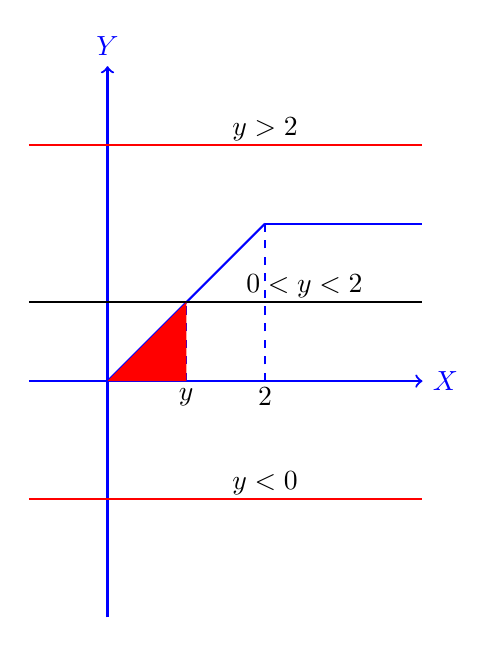
\begin{tikzpicture}
        \draw[blue, thick, ->] (-1,0) -- (4,0) node[right] {$X$};
        \draw[blue, thick, ->] (0,-3) -- (0,4) node[above] {$Y$};
        \draw[blue, thick](0,0) -- (2,2);
        \draw[blue, thick](2,2) --(4,2);
        \draw[blue, thick, dashed] (2,0)--(2,2);
        \node at (2,-0.2) {$2$};
        \draw[red, thick](-1,-1.5) -- (4, -1.5);
        \node at (2, -1.3) {$y<0$};
        \draw[red, thick](-1, 3) --(4, 3);
        \node at (2, 3.2) {$y>2$};
        \draw[black, thick](-1,1) -- (4, 1);
        \draw[blue, thick, dashed](1,0)--(1,1);
        \fill[red](0,0)--(1,1)--(1,0)--(0,0);
        \node at (2.5, 1.2) {$0<y<2$};
        \node at (1,-0.2) {$y$};
    \end{tikzpicture}
    \end{center}
    故$F_Y(y)={\min{\{X,2\}}<y}$,当$y<0$时候$F_Y(y)=0$,$y\geq 2$,$F_Y(y)=1$,当$0\leq y<2$时候,有
    $\int_{0}^{y}f(x)dx=1-e^{-\lambda y}$,综上
    \[
    F_Y=\begin{cases}
        0, &y<0 \\
        1-e^{-\lambda y}, &0\leq y < 2\\
        1, &y\geq 2
    \end{cases}
    \]
    容易发现$F(2-0)\neq 1$故存在一个跳跃间断点
    \end{solution}
    
    % 例题2.16
    \item  设随机变量$X$的概率密度为
    $f(x)=\begin{cases}
        \frac{x^2}{a}, & 0<x<3 \\
        0, & \text{其他}
    \end{cases}$
    $Y=\begin{cases}
        2, & X\leq 1 \\
        X, & 1<X<2 \\
        1, & X\geq 2
    \end{cases}$
    \begin{enumerate}
        \item 求$Y$的分布函数;
        \item 求$P\{X\leq Y\}$.
    \end{enumerate}
    
    \begin{solution}
    带参数的概率密度第一步就应该根据正则性把这个参数求出来.$$\int_{0}^{3}f(x)dx=1\implies a = 9$$
    然后和上一题一样画$X-Y$图像,求$F_Y(y)$,注意分区域就是.
    \begin{center}
    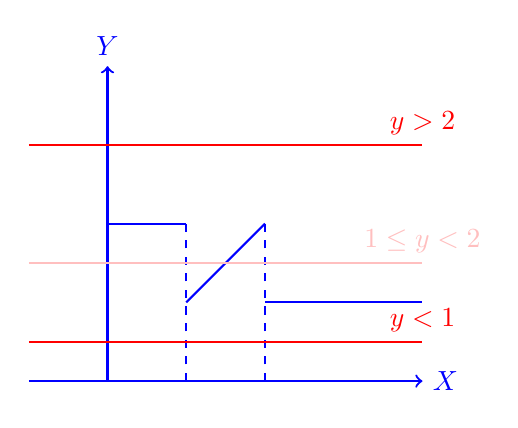
\begin{tikzpicture}
        \draw[blue, thick, ->] (-1,0)--(4,0) node[right] {$X$};
        \draw[blue, thick, ->] (0,0)--(0,4) node[above] {$Y$};
        \draw[blue, thick] (0,2)--(1,2);
        \draw[blue, thick] (1,1)--(2,2);
        \draw[blue, thick] (2,1)--(4,1);
        \draw[blue, thick, dashed] (1,0)--(1,2);
        \draw[blue, thick, dashed] (2,0)--(2,2);
        \draw[red, thick](-1,3)--(4,3) node[above] {$y>2$};
        \draw[red, thick](-1,0.5)--(4,0.5) node[above] {$y<1$};
        \draw[pink, thick](-1,1.5)--(4,1.5) node[above] {$1\leq y < 2$};
    \end{tikzpicture}
    \end{center}
    当$y<1,F_Y(y)=0;y>2,F_Y(y)=1$ \\
    $1\leq y < 2, F_Y(y)=\int_{1}^{y}f(x)dx+\int_{2}^{3}f(x)dx=\frac{y^3}{27}+\frac{2}{3}$
    \end{solution}
    
    % 例题2.17
    \item  (2021,数一、三)在区间$(0,2)$上随机取一点,将该区间分成两段,较短一段的长度记为$X$,较长一段的长度记为$Y$。
    \begin{enumerate}
        \item 求$X$的概率密度;
        \item 求$Z=\frac{Y}{X}$的概率密度;
        \item 求$E\left(\frac{Y}{X}\right)$.
    \end{enumerate}
    
    \begin{solution}
    有题设容易得到$X\sim U(0,1),Y=2-X$
    \item [(1)] 则$f(x)=\begin{cases}
        1, &x\in (0,1) \\
        0, &\text{其他}
    \end{cases}$
    \item [(2)] $Z=\frac{Y}{X}=\frac{2}{X}-1$,显然Z关于X是单调的,可以用公式法直接求出$f_{Z}(z)$,即
    \[
    f_Z(z)=1\cdot \frac{2}{(y+1)^2} =\frac{2}{(y+1)^2},z\in (1,+\infty)
    \]
    \item [(3)] 
    \[
    E(Z)=\int_{1}^{\infty}zf_{Z}(z)dz=2\ln{2}-1
    \]
    或者也可以用
    \[
    E(\frac{2}{x}-1)=\int_{0}^{1}(\frac{2}{x}-1)dx = 2\ln(2) - 1
    \]
    \end{solution}
\end{enumerate}

\ifx\allfiles\undefined
\end{document}
\fi